\documentclass[border=10pt]{standalone}
\usepackage{pgfplots}
\pgfplotsset{compat=1.18}
\begin{document}
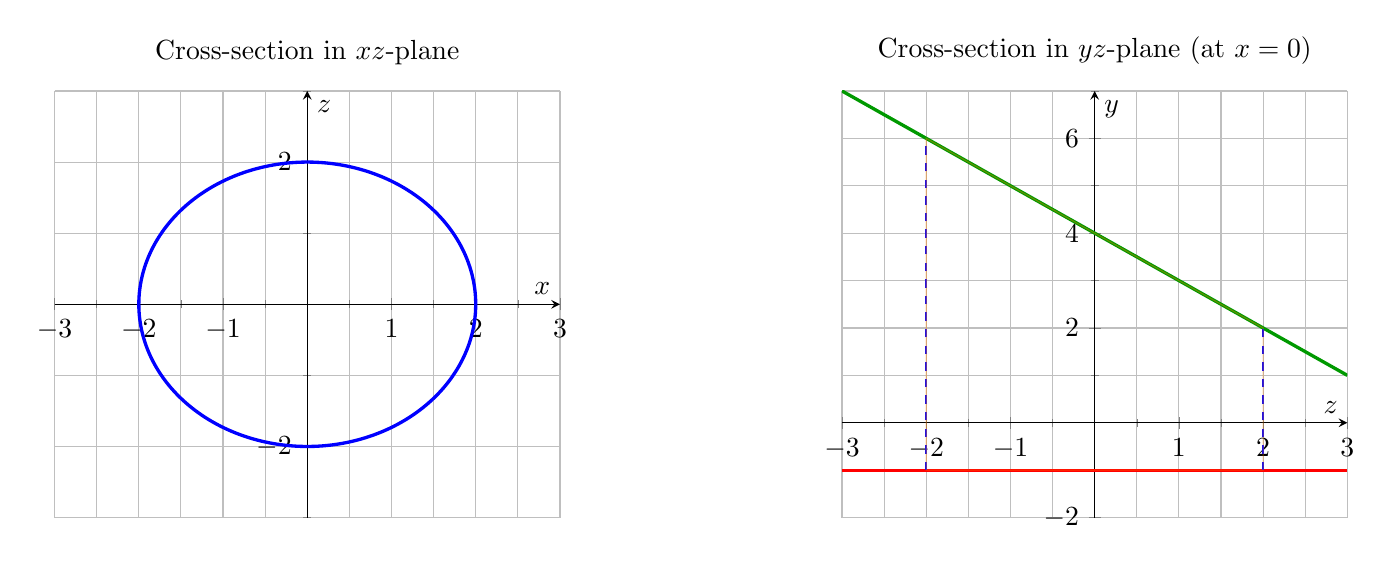
\begin{tikzpicture}
% Left: xz-plane disk
\begin{axis}[
    at={(0,0)}, anchor=center,
    xlabel={$x$}, ylabel={$z$},
    xmin=-3, xmax=3, ymin=-3, ymax=3,
    axis lines=middle, grid=both, minor tick num=1,
    title={Cross-section in $xz$-plane},
    width=8cm, height=7cm
]
\addplot[blue, very thick, domain=0:360, samples=120, smooth] ({2*cos(x)},{2*sin(x)});
\end{axis}

% Right: yz-plane
\begin{axis}[
    at={(10cm,0)}, anchor=center,
    xlabel={$z$}, ylabel={$y$},
    xmin=-3, xmax=3, ymin=-2, ymax=7,
    axis lines=middle, grid=both, minor tick num=1,
    title={Cross-section in $yz$-plane (at $x=0$)},
    width=8cm, height=7cm
]
\addplot[red, very thick, domain=-3:3] ({x},{-1});
\addplot[green!60!black, very thick, domain=-3:3] ({x},{4-x});
\addplot[blue, dashed, thick] coordinates {(-2,-1) (-2,6)};
\addplot[blue, dashed, thick] coordinates {(2,-1) (2,2)};
\addplot[orange, opacity=0.4] coordinates {(-2,-1) (2,-1) (2,2) (-2,6)} -- cycle;
\end{axis}
\end{tikzpicture}
\end{document}